\documentclass[addpoints, 11pt]{exam}
\usepackage[a4paper, left=20mm, right=20mm, top=26mm, bottom=30mm, headsep=6mm, footskip=12mm, headheight=15pt]{geometry}
\usepackage[T1]{fontenc}
\usepackage[utf8]{inputenc}
\usepackage{lmodern}
\usepackage{textcomp}
\usepackage[french]{babel}
\usepackage{xcolor}
\usepackage{listings}
\usepackage{graphicx}
\usepackage{array}
\usepackage{amsmath}
\usepackage{eurosym}
\usepackage{needspace}
\usepackage[most]{tcolorbox}
\usepackage{tikz}
\usetikzlibrary{positioning,arrows.meta}


% --- Code Python : même style que le sujet, en police à chasse fixe ---
\definecolor{codegreen}{rgb}{0,0.6,0}
\definecolor{codegray}{rgb}{0.5,0.5,0.5}
\definecolor{codepurple}{rgb}{0.58,0,0.82}
\definecolor{backcolour}{rgb}{0.95,0.95,0.92}
\lstdefinestyle{mystyle}{
    backgroundcolor=\color{backcolour},
    commentstyle=\color{codegreen},
    keywordstyle=\color{magenta},
    numberstyle=\tiny\color{codegray},
    stringstyle=\color{codepurple},
    basicstyle=\footnotesize\ttfamily,
    columns=fullflexible,
    breakatwhitespace=false,
    breaklines=true,
    postbreak=\mbox{\textcolor{codegray}{$\hookrightarrow$}\space},
    captionpos=b,
    keepspaces=true,
    numbers=left,
    numbersep=5pt,
    xleftmargin=1.5em,
    showspaces=false,
    showstringspaces=false,
    showtabs=false,
    tabsize=4,
    upquote=true
}
\lstset{style=mystyle, language=Python, extendedchars=true,
  literate={à}{{\`a}}1 {â}{{\^a}}1 {ä}{{\"a}}1 {ç}{{\c{c}}}1
           {é}{{\'e}}1 {è}{{\`e}}1 {ê}{{\^e}}1 {ë}{{\"e}}1
           {î}{{\^i}}1 {ï}{{\"i}}1 {ô}{{\^o}}1 {ö}{{\"o}}1
           {ù}{{\`u}}1 {û}{{\^u}}1 {ü}{{\"u}}1 {œ}{{\oe}}2
           {É}{{\'E}}1 {È}{{\`E}}1 {À}{{\`A}}1 {Ç}{{\c{C}}}1
           {°}{{\textdegree}}1 {€}{{\euro}}1 {…}{{\dots}}1
           {«}{{\guillemotleft}}1 {»}{{\guillemotright}}1 {·}{{\textperiodcentered}}1}
% Terminal (commandes Linux) : sans couleur de mots-clés
\lstdefinestyle{terminal}{style=mystyle, language={}, numbers=none, xleftmargin=0.5em}
% Sortie d'un programme (ce qui s'affiche à l'écran)
\lstdefinestyle{sortie}{style=mystyle, language={}, numbers=none, backgroundcolor=\color{white}, frame=single, rulecolor=\color{black!60}, xleftmargin=0.5em}

% --- Boîtes du corrigé (lisibles en noir et blanc) ---
\newtcolorbox{reponse}[1][Réponse attendue]{enhanced, breakable, colback=white, colframe=black, boxrule=1.2pt, arc=0pt,
  fonttitle=\bfseries, coltitle=white, colbacktitle=black, title=#1, left=2mm, right=2mm, top=1mm, bottom=1mm, before skip=6pt, after skip=6pt}
\newtcolorbox{erreur}[1][Erreur fréquente]{enhanced, breakable, colback=black!6, colframe=black!55, boxrule=0.6pt, arc=2pt,
  borderline west={3pt}{0pt}{black!70}, fonttitle=\bfseries, coltitle=black, colbacktitle=black!15, title=#1, left=2mm, right=2mm, top=1mm, bottom=1mm, before skip=6pt, after skip=6pt}
\newtcolorbox{astuce}[1][À retenir]{enhanced, breakable, colback=white, colframe=black!55, boxrule=0.6pt, arc=2pt,
  fonttitle=\bfseries, coltitle=black, colbacktitle=black!8, title=#1, left=2mm, right=2mm, top=1mm, bottom=1mm, before skip=6pt, after skip=6pt}
\newtcolorbox{remarque}[1][Remarque sur l'énoncé]{enhanced, breakable, colback=white, colframe=black!70, boxrule=0.6pt, arc=0pt,
  borderline={0.4pt}{1.2pt}{black!70, dashed}, fonttitle=\bfseries, coltitle=black, colbacktitle=white, title=#1, left=2mm, right=2mm, top=1mm, bottom=1mm, before skip=6pt, after skip=6pt}
\newcommand{\enonce}[1]{\textit{#1}\par\smallskip}
\newcommand{\methode}{\par\smallskip\noindent\textbf{Méthode.}\ }
\newcommand{\explication}{\par\smallskip\noindent\textbf{Explication.}\ }
\newcommand{\code}[1]{\texttt{#1}}
% Coupure de ligne possible après un tiret bas (noms de variables longs)
\DeclareRobustCommand{\_}{\textunderscore\allowbreak}
% Un code court ne se coupe pas en bas de page
\AddToHook{env/lstlisting/before}{\needspace{10\baselineskip}}
\setlength{\parindent}{0pt}
\setlength{\parskip}{3pt}
\renewcommand{\arraystretch}{1.25}

\title{Corrigé --- Examen Première NSI - Listes}
\author{Babash - NSI Tani Malandi et Johanne Bakalara}
\date{}

\begin{document}
\pagestyle{headandfoot}
\runningheader{}{}{\footnotesize Corrigé --- Listes}
\firstpageheader{}{}{}
\runningfooter{}{\footnotesize Babash - NSI Tani Malandi et Johanne Bakalara \textperiodcentered{} CC BY-SA 4.0 \textperiodcentered{} page \thepage}{}
\firstpagefooter{}{\footnotesize Babash - NSI Tani Malandi et Johanne Bakalara \textperiodcentered{} CC BY-SA 4.0 \textperiodcentered{} page \thepage}{}

\maketitle
\thispagestyle{headandfoot}

\begin{astuce}[Comment lire ce corrigé]
Pour chaque question : la question est rappelée en italique, puis la \textbf{réponse attendue} est encadrée en noir, puis l'\textbf{explication} montre la méthode, étape par étape.
Les encadrés gris « Erreur fréquente » signalent les pièges les plus courants. Essaie d'abord de refaire la question seul·e, puis compare ta démarche avec celle du corrigé.
\end{astuce}

\section*{Barème}
\begin{center}
  \gradetable[h]
\end{center}

\begin{questions}

% =====================================================================
\section{Listes : manipulations élémentaires}

\question[4] \enonce{Questions de cours.}
\begin{parts}
\part \enonce{Créer une variable \code{l} de type liste contenant 1, 3 et 5.}
\begin{reponse}
\lstinline!l = [1, 3, 5]!
\end{reponse}
Une liste s'écrit entre \textbf{crochets}, les éléments séparés par des virgules.

\part \enonce{Quelle commande affiche la longueur de \code{l} ?}
\begin{reponse}
\lstinline!print(len(l))!
\end{reponse}
\code{len(l)} \textbf{calcule} la longueur (le nombre d'éléments) ; \code{print} l'\textbf{affiche}. Pour \code{[1, 3, 5]}, on voit 3.

\part \enonce{Avec \code{l = [4, 2, 9]}, que vaut \code{l[2]} ?}
\begin{reponse}
\code{l[2]} vaut \textbf{9}.
\end{reponse}
Les indices commencent à \textbf{0} :
\begin{center}
\begin{tabular}{|l|c|c|c|}
\hline
Élément & 4 & 2 & 9 \\ \hline
Indice positif & 0 & 1 & 2 \\ \hline
Indice négatif & $-3$ & $-2$ & $-1$ \\ \hline
\end{tabular}
\end{center}
\begin{erreur}
Répondre 2 en pensant « le 2\textsuperscript{e} élément ». \code{l[2]} est le \textbf{3\textsuperscript{e}} élément, car le premier est \code{l[0]}.
\end{erreur}

\part \enonce{Que vaut \code{l[-2]} ?}
\begin{reponse}
\code{l[-2]} vaut \textbf{2}.
\end{reponse}
Un indice négatif compte \textbf{depuis la fin} : \code{l[-1]} est le dernier élément (9), \code{l[-2]} l'avant-dernier (2).

\part \enonce{Que vaut \code{4 in l} ?}
\begin{reponse}
\code{True}
\end{reponse}
\code{in} teste si une valeur est \textbf{présente} dans la liste et renvoie un booléen. 4 est bien dans \code{[4, 2, 9]}.

\part \enonce{Que se passe-t-il avec \code{l[5]} ? Expliquer.}
\begin{reponse}
Python affiche une erreur : \code{IndexError: list index out of range} (« indice de liste hors limites »). La liste a 3 éléments, d'indices 0 à 2 : l'indice 5 n'existe pas.
\end{reponse}
Le plus grand indice possible est toujours \code{len(l) - 1}. Python ne « devine » pas de valeur : il arrête le programme et signale l'erreur.

\part \enonce{Après \code{l.append(12)}, que vaut \code{l} ?}
\begin{reponse}
\code{[4, 2, 9, 12]}
\end{reponse}
\code{append} ajoute l'élément \textbf{à la fin} de la liste. La liste est modifiée directement.

\part \enonce{Après \code{l.insert(1, 3)}, que vaut \code{l} ?}
\begin{reponse}
\code{[4, 3, 2, 9, 12]}
\end{reponse}
\code{insert(position, valeur)} : le \textbf{premier} nombre est la position, le second la valeur. On insère donc la valeur 3 à l'indice 1 ; les éléments suivants sont décalés vers la droite. On part de la liste modifiée par \code{append} à la question précédente.
\begin{erreur}
Inverser les deux arguments et insérer 1 à l'indice 3 : on obtiendrait \code{[4, 2, 9, 1, 12]}.
\end{erreur}
\end{parts}

% =====================================================================
\needspace{14\baselineskip}
\section{Listes : compréhension de code}

\begin{lstlisting}
def multiplication(tab1, tab2):
    # On verifie que tab1 et tab2 sont de meme taille
    assert len(tab1) == len(tab2)
    res = 0
    for i in range(len(tab1)):
        res += tab1[i]*tab2[i]
    return res
\end{lstlisting}

\question[1] \enonce{Quel type de parcours est présent dans ce code ?}
\begin{reponse}
Un \textbf{parcours par indice} (ou par index).
\end{reponse}
La boucle \code{for i in range(len(tab1))} fait varier \code{i} sur les positions 0, 1, 2\dots, et on lit les éléments avec \code{tab1[i]} et \code{tab2[i]}. Ici, c'est indispensable : on a besoin de la \textbf{même position} dans deux listes à la fois. Un parcours par valeur (\code{for v in tab1}) ne donnerait pas accès à l'élément correspondant de \code{tab2}.

\question[3] \enonce{Compléter le tableau d'avancement pour \code{multiplication([10, 100, 8, 4, 1], [2, 3, 1, 5, 2])}.}
\begin{reponse}
\begin{center}
\begin{tabular}{|c|c|c|c|c|c|}
\hline
Tour & \code{i} & \code{tab1[i]} & \code{tab2[i]} & \code{tab1[i]*tab2[i]} & \code{res} \\ \hline
Avant & & & & & 0 \\
0 & 0 & 10 & 2 & 20 & 20 \\
1 & 1 & 100 & 3 & 300 & 320 \\
2 & 2 & 8 & 1 & 8 & 328 \\
3 & 3 & 4 & 5 & 20 & 348 \\
4 & 4 & 1 & 2 & 2 & 350 \\ \hline
\multicolumn{6}{|l|}{Retour : \textbf{350}} \\ \hline
\end{tabular}
\end{center}
\end{reponse}
\methode
\begin{enumerate}
  \item Avant la boucle : l'\code{assert} vérifie que les deux listes ont la même taille (5 et 5 : c'est bon, le programme continue), puis \code{res = 0}.
  \item À chaque tour : lire les deux éléments à l'indice \code{i}, les multiplier, puis ajouter le produit à \code{res}. \code{res += x} veut dire \code{res = res + x}.
  \item \code{range(5)} donne 0 à 4 : 5 tours. Après le dernier, la fonction renvoie \code{res}.
\end{enumerate}
\textit{Pour aller plus loin :} cette fonction calcule ce qu'on appelle en mathématiques le \textbf{produit scalaire} de deux vecteurs.

\question[2] \enonce{Donner la valeur de retour pour chaque appel (sans tableau).}
\begin{reponse}
\begin{tabular}{ll}
\code{multiplication([0, 0, \dots, 0], [10, 10, \dots, 10])} : & \textbf{0}\\
\code{multiplication([1, 1, 1, 1, 1, 1], [1, 2, 3, 4, 5, 6])} : & \textbf{21}\\
\code{multiplication([2, 3, 4], [7, 8, 9])} : & \textbf{74}\\
\code{multiplication([1 for i in range(5)], [i for i in range(5)])} : & \textbf{10}\\
\end{tabular}
\end{reponse}
\begin{enumerate}
  \item Tous les produits valent $0 \times 10 = 0$ : la somme est 0.
  \item Multiplier par 1 ne change rien : on additionne $1 + 2 + 3 + 4 + 5 + 6 = 21$.
  \item $2 \times 7 + 3 \times 8 + 4 \times 9 = 14 + 24 + 36 = 74$.
  \item Ces listes sont écrites \textbf{en compréhension} : \code{[1 for i in range(5)]} donne \code{[1, 1, 1, 1, 1]} (un 1 pour chaque \code{i}) et \code{[i for i in range(5)]} donne \code{[0, 1, 2, 3, 4]}. On calcule donc $0 + 1 + 2 + 3 + 4 = 10$.
\end{enumerate}

% =====================================================================
\section{Listes : concevoir des algorithmes avec des listes}

\question[3] \enonce{Compléter la fonction \code{filtre\_pair\_impair}, qui renvoie la liste des nombres pairs et la liste des nombres impairs.}
\begin{reponse}
\begin{lstlisting}
def filtre_pair_impair(tab):
    pairs = []      # on crée une liste vide pair
    impairs = []    # on crée une liste vide impair
    for v in tab:   # on parcourt tab par valeur
        if v%2 == 0 :   # si v est pair
            pairs.append(v)     # on ajoute v à la liste pair
        else :
            impairs.append(v)   # on ajoute v à la liste impair
    return pairs, impairs
\end{lstlisting}
\end{reponse}
\explication
\begin{itemize}
  \item Lignes 2 et 3 : une liste vide s'écrit \code{[]}.
  \item Ligne 4 : « par valeur » : on parcourt directement \code{tab}, et \code{v} prend chaque nombre.
  \item Lignes 6 et 8 : \code{append} ajoute \code{v} à la fin de la bonne liste.
\end{itemize}
\textbf{Trace de} \code{filtre\_pair\_impair([1, 2, 3, 4, 5, 6])} :
\begin{center}
\begin{tabular}{|c|c|c|l|l|}
\hline
\code{v} & \code{v\%2} & pair ? & \code{pairs} & \code{impairs} \\ \hline
& & & \code{[]} & \code{[]} \\
1 & 1 & non & \code{[]} & \code{[1]} \\
2 & 0 & oui & \code{[2]} & \code{[1]} \\
3 & 1 & non & \code{[2]} & \code{[1, 3]} \\
4 & 0 & oui & \code{[2, 4]} & \code{[1, 3]} \\
5 & 1 & non & \code{[2, 4]} & \code{[1, 3, 5]} \\
6 & 0 & oui & \code{[2, 4, 6]} & \code{[1, 3, 5]} \\ \hline
\end{tabular}
\end{center}
La fonction renvoie \code{([2, 4, 6], [1, 3, 5])}.
\begin{erreur}
Écrire \code{pairs = pairs.append(v)} : \code{append} modifie la liste et renvoie \code{None}, donc \code{pairs} deviendrait \code{None}. On écrit simplement \code{pairs.append(v)}.
\end{erreur}

% =====================================================================
\section{Problème}

\begin{astuce}[À retenir : la grille]
Une case se note par une \textbf{lettre} (la ligne, de A en haut à O en bas) et un \textbf{nombre} (la colonne, de 1 à gauche à 15 à droite). Le robot part de \textbf{H8}, au centre.
\begin{itemize}
  \item \code{droite(x)} augmente le numéro de colonne de \code{x} ; \code{gauche(x)} le diminue.
  \item \code{haut(x)} remonte de \code{x} lettres (H $\to$ G $\to$ F\dots) ; \code{bas(x)} descend de \code{x} lettres.
\end{itemize}
Exemple du sujet : \code{droite(1)} : H8 $\to$ H9 ; \code{haut(3)} : H9 $\to$ E9 ; \code{gauche(2)} : E9 $\to$ E7.
\end{astuce}

\question[1] \enonce{Écrire les instructions qui emmènent le robot de H8 à G15.}
\begin{reponse}
\begin{lstlisting}
haut(1)
droite(7)
\end{lstlisting}
Parcours : H8 -- G8 -- G15.
\end{reponse}
\methode\ On calcule séparément le déplacement vertical et le déplacement horizontal.
\begin{enumerate}
  \item Lignes : de H à G, on remonte d'\textbf{une} lettre : \code{haut(1)}.
  \item Colonnes : de 8 à 15, on va à droite de $15 - 8 = 7$ : \code{droite(7)}.
\end{enumerate}
L'ordre inverse (\code{droite(7)} puis \code{haut(1)}) est aussi juste : on passe alors par H15.

\question[4] \enonce{Donner le parcours du robot, déplacement par déplacement, pour chaque code.}
\begin{parts}
\part
\begin{lstlisting}
D = [3, 4, 1, 2]
a = 2
droite(D[a])
haut(D[1])
a = 1
bas(D[a])
\end{lstlisting}
\begin{reponse}
H8 -- H9 -- D9 -- H9
\end{reponse}
\code{D[2]} vaut 1 : \code{droite(1)} mène en H9. \code{D[1]} vaut 4 : \code{haut(4)} mène en D9 (H, G, F, E, D). Puis \code{a} vaut 1, donc \code{D[a]} vaut 4 : \code{bas(4)} ramène en H9.
\begin{erreur}
Lire \code{D[2]} comme le 2\textsuperscript{e} élément (4). L'indice 2 désigne le 3\textsuperscript{e} élément : 1.
\end{erreur}

\part
\begin{lstlisting}
D = [[3, 4],[1, 2]]
for i in range(len(D)):
    gauche(D[i][0])
    haut(D[i][1])
\end{lstlisting}
\begin{reponse}
H8 -- H5 -- D5 -- D4 -- B4
\end{reponse}
\code{D} est une \textbf{liste de listes} de longueur 2 : deux tours.
\begin{center}
\begin{tabular}{|c|c|c|c|l|}
\hline
\code{i} & \code{D[i]} & \code{D[i][0]} & \code{D[i][1]} & Déplacements \\ \hline
0 & \code{[3, 4]} & 3 & 4 & \code{gauche(3)} : H5 ; \code{haut(4)} : D5 \\
1 & \code{[1, 2]} & 1 & 2 & \code{gauche(1)} : D4 ; \code{haut(2)} : B4 \\ \hline
\end{tabular}
\end{center}

\part
\begin{lstlisting}
D = [3, 3, 4, 1, 2, 1]
for i in range(len(D)-1):
    if D[i] - D[i+1] > 0:
        gauche(D[i])
    elif D[i] - D[i+1] < 0:
        droite(D[i])
    else:
        haut(D[i])
\end{lstlisting}
\begin{reponse}
H8 -- E8 -- E11 -- E7 -- E8 -- E6
\end{reponse}
\code{len(D) - 1} vaut 5 : \code{i} va de 0 à 4. On compare chaque élément avec le \textbf{suivant}.
\begin{center}
\begin{tabular}{|c|c|c|c|l|c|}
\hline
\code{i} & \code{D[i]} & \code{D[i+1]} & \code{D[i] - D[i+1]} & Instruction & Case \\ \hline
0 & 3 & 3 & 0 & \code{haut(3)} & E8 \\
1 & 3 & 4 & $-1$ & \code{droite(3)} & E11 \\
2 & 4 & 1 & 3 & \code{gauche(4)} & E7 \\
3 & 1 & 2 & $-1$ & \code{droite(1)} & E8 \\
4 & 2 & 1 & 1 & \code{gauche(2)} & E6 \\ \hline
\end{tabular}
\end{center}
Attention : on se déplace de \code{D[i]} cases, pas de la différence.

\part
\begin{lstlisting}
D = [3, 3, 4, 1, 2, 1]
for v in D:
    if colonne() > v:
        gauche(v)
    else:
        droite(v)
\end{lstlisting}
\begin{reponse}
H8 -- H5 -- H2 -- H6 -- H5 -- H3 -- H2
\end{reponse}
Ici, le parcours est \textbf{par valeur} : \code{v} prend les 6 valeurs de \code{D}. \code{colonne()} donne la colonne actuelle ; elle change après chaque déplacement.
\begin{center}
\begin{tabular}{|c|c|c|l|c|}
\hline
\code{v} & \code{colonne()} & \code{colonne() > v} ? & Instruction & Case \\ \hline
3 & 8 & vrai & \code{gauche(3)} & H5 \\
3 & 5 & vrai & \code{gauche(3)} & H2 \\
4 & 2 & faux & \code{droite(4)} & H6 \\
1 & 6 & vrai & \code{gauche(1)} & H5 \\
2 & 5 & vrai & \code{gauche(2)} & H3 \\
1 & 3 & vrai & \code{gauche(1)} & H2 \\ \hline
\end{tabular}
\end{center}
Le robot reste sur la ligne H : il ne fait que des déplacements à gauche ou à droite.
\end{parts}

\begin{center}
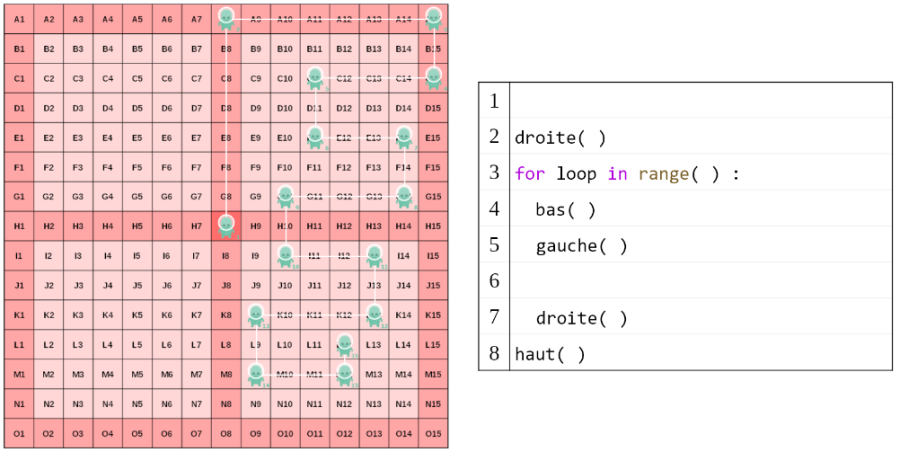
\includegraphics[width=0.45\linewidth, trim= {0 0 325 0}, clip]{BLOB/exoinverse-f268d.png}\\
{\footnotesize Capture d\textquoteright Alien-Python (Mathieu Degrange, MIT) ; alien : Kenney (CC0).}
\end{center}

\question[1] \enonce{Écrire un code qui fait le parcours de l'image.}
\begin{reponse}
\begin{lstlisting}
haut(7)
droite(7)
bas(2)
gauche(4)
bas(2)
droite(3)
bas(2)
gauche(4)
bas(2)
droite(3)
bas(2)
gauche(4)
bas(2)
droite(3)
haut(1)
\end{lstlisting}
\end{reponse}
\methode\ Suivre les numéros de l'image (de 1 à 16) et écrire un déplacement pour chaque segment :
H8 $\to$ A8 (\code{haut(7)}) $\to$ A15 (\code{droite(7)}) $\to$ C15 (\code{bas(2)}) $\to$ C11 (\code{gauche(4)}) $\to$ E11 (\code{bas(2)}) $\to$ E14 (\code{droite(3)}) $\to$ G14 $\to$ G10 $\to$ I10 $\to$ I13 $\to$ K13 $\to$ K9 $\to$ M9 $\to$ M12 $\to$ L12 (\code{haut(1)}).
Pour compter, fais la différence des numéros de colonne (15 $-$ 11 $= 4$) ou compte les lettres (C, D, E : on descend de 2).

\question[1] \enonce{Écrire un autre code de moins de 10 lignes pour le même parcours.}
\begin{reponse}
\begin{lstlisting}
haut(7)
droite(7)
for loop in range(3):
    bas(2)
    gauche(4)
    bas(2)
    droite(3)
haut(1)
\end{lstlisting}
\end{reponse}
\methode
\begin{enumerate}
  \item Dans le code précédent, chercher un \textbf{motif qui se répète} : \code{bas(2)}, \code{gauche(4)}, \code{bas(2)}, \code{droite(3)} apparaît 3 fois de suite.
  \item Mettre ce motif dans une boucle \code{for} qui tourne 3 fois : \code{range(3)}.
  \item Garder hors de la boucle ce qui ne se répète pas : le début (\code{haut(7)}, \code{droite(7)}) et la fin (\code{haut(1)}).
\end{enumerate}
On obtient 8 lignes, et le même parcours (vérifié en simulant les deux codes) : on termine bien en L12.
\begin{erreur}
Mettre \code{haut(1)} dans la boucle (indenté) : il serait exécuté 3 fois, et le robot ne suivrait plus le chemin.
\end{erreur}

\end{questions}

\end{document}
